% \documentclass[14pt]{beamer}
\documentclass{beamer}
% \documentclass[aspectratio=169]{beamer}

\usetheme{Copenhagen}
% \usetheme{Boadilla}
% \usecolortheme{beaver}
\setbeamercolor{alerted text}{fg=orange}
\setbeamercolor{background canvas}{bg=white}
\setbeamercolor{block body alerted}{bg=normal text.bg!90!black}
\setbeamercolor{block body}{bg=normal text.bg!90!black}
\setbeamercolor{block body example}{bg=normal text.bg!90!black}
\setbeamercolor{block title alerted}{use={normal text,alerted text},fg=alerted text.fg!75!normal text.fg,bg=normal text.bg!75!black}
% \setbeamercolor{block title}{bg=blue}
\setbeamercolor{block title example}{use={normal text,example text},fg=example text.fg!75!normal text.fg,bg=normal text.bg!75!black}
\setbeamercolor{fine separation line}{}
\setbeamercolor{frametitle}{fg=white}
\setbeamercolor{item projected}{fg=white}
\setbeamercolor{normal text}{bg=white,fg=black}
\setbeamercolor{palette sidebar primary}{use=normal text,fg=normal text.fg}
\setbeamercolor{palette sidebar quaternary}{use=structure,fg=structure.fg}
\setbeamercolor{palette sidebar secondary}{use=structure,fg=structure.fg}
\setbeamercolor{palette sidebar tertiary}{use=normal text,fg=normal text.fg}
\setbeamercolor{section in sidebar}{fg=brown}
\setbeamercolor{section in sidebar shaded}{fg=grey}
\setbeamercolor{separation line}{}
\setbeamercolor{sidebar}{bg=red}
\setbeamercolor{sidebar}{parent=palette primary}

\setbeamercolor{structure}{bg=black, fg=white!30!blue!70!green}

\setbeamercolor{subsection in sidebar}{fg=brown}
\setbeamercolor{subsection in sidebar shaded}{fg=grey}
\setbeamercolor{title}{fg=white}
\setbeamercolor{titlelike}{fg=white}

\setbeamerfont{bibliography item}{size=\tiny}
\setbeamerfont{bibliography entry author}{size=\tiny}
\setbeamerfont{bibliography entry title}{size=\tiny}
\setbeamerfont{bibliography entry location}{size=\tiny}
\setbeamerfont{bibliography entry note}{size=\tiny}

% Szép kék
% \setbeamercolor{structure}{bg=black, fg=white!10!green!40!blue}

\frenchspacing

% Language packages
\usepackage[utf8]{inputenc}
\usepackage[T1]{fontenc}
\usepackage[magyar]{babel}

% AMS
\usepackage{amssymb,amsmath}

% Graphic packages
\usepackage{graphicx}

% Syntax highlighting
\usepackage{listings}

\usepackage{tikz}

\title[Szakdolgozat védés, 2020. június 23.]{\Huge Kiterjesztett valóság alapú prezentációs szoftver készítése}
\subtitle{\bigskip \large Témavezető: \textbf{\Large Piller Imre}}
\author[Nagy Dániel Zoltán]{\textbf{\LARGE Nagy Dániel Zoltán}}
\institute[]{\Large Miskolci Egyetem}
\date{2020. június 23.}

% ==============
\begin{document}
% ==============

% --------------------
\frame{\Large \titlepage}

% --------------------
\begin{frame}[fragile]
\frametitle{Feladat}

AR alapú prezentációs szoftver készítése, melyben a prezentáló személy a prezentáció menetét a videófolyamon megjelenő virtuális vezérlők segítségével iránythatja. A programmal a gesztusai segítségével léphet kapcsolatba.

\medskip
\begin{block}{}
\begin{itemize}
	\item Videófolyam feldolgozása
	\item Gesztusok definiálása, detektálásának módjai
	\item Szükséges vezérlők tervezése, megjelenítésük
	\item Prezentációt leíró állomány kialakítása
\end{itemize}
\end{block}

\medskip


\includegraphics[width=\textwidth]{images/globe.png}

\end{frame}

% --------------------
\begin{frame}[fragile]
\frametitle{Feladat}

\begin{columns}
    \begin{column}{4cm}
		\begin{figure}[htb]
			
\includegraphics[height=3cm]{images/OpenCV-logo.png}
			
			\bigskip
			
			
\includegraphics[height=2cm]{images/scikit-learn-logo.png}
		\end{figure}
    \end{column}

    \begin{column}{7cm}
    		\textbf{Képfeldolgozás - OpenCV} \cite{bradski2008learning}
		\begin{itemize}
    			\item Magas tudású függvénykönyvtár
    			\item Számos képfeldolgozó algoritmus
    			\item Valós idejű videó feldolgozás
			\item Platformfüggetlen
		\end{itemize}
		\bigskip
		\textbf{Gépi tanulás - Scikit Learn} \cite{pedregosa2011scikit}
		\begin{itemize}
    			\item Python környezethez
    			\item Könnyen használható API
    			\item Osztályozás, klaszterezés, regresszió
		\end{itemize}
    \end{column}
\end{columns}

\end{frame}

% --------------------
\begin{frame}[fragile]
\frametitle{Követelmények egy ilyen jellegű programmal szemben}
\begin{figure}[htb]
	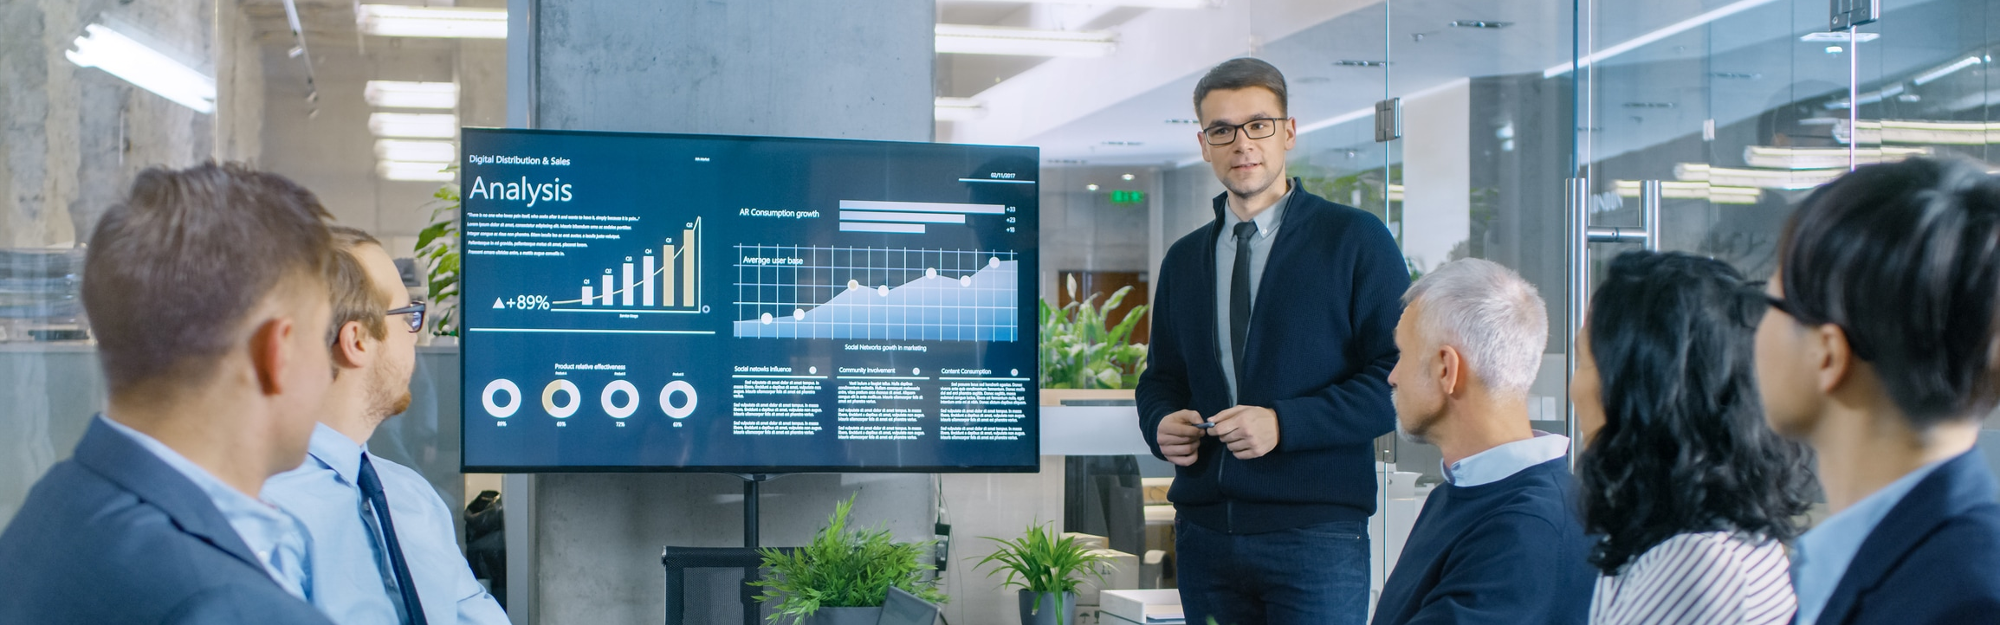
\includegraphics[width=\textwidth]{images/presentation_stock_photo.png}
\end{figure}
\begin{block}{}
\begin{itemize}
	\item Valós és virtuális elemek keverése, megjelenítése
	\item Interakció lehetősége a virtuális elemekkel
	\item Témakör látványos bemutathatósága
	\item Gesztusfelismerés
	\item Könnyű használat
\end{itemize}
\end{block}

\end{frame}

% --------------------
\begin{frame}[fragile]
\frametitle{Követelmények egy ilyen jellegű programmal szemben}

\begin{block}{Nehézségek}
\begin{itemize}
	\item Technikai korlátok
	\item Eszközfüggőség minimalizálása
	\item Valós idejű futás biztosítása
	\item A prezentáló személy mozdulatainak pontos feldolgozása
	\item A vezérlők kényelmes, természetes használatának biztosítása
\end{itemize}
\end{block}
\begin{figure}[htb]
	
\includegraphics[width=\textwidth]{images/harold.png}
\end{figure}

\end{frame}

% --------------------
\begin{frame}[fragile]
\frametitle{Mozgás érzékelése}

\textbf{Kulcs feladat:}\\
Mozgás érzékelése, megfigyelése, mozgásinformációk gyűjtése

\medskip

\begin{block}{Példák a probléma megközelítésére}
\begin{itemize}
	\item Deep-Learning alapú alakfelismerés \cite{cao2018openpose}
	\item Különféle technikák segítségével azonosítani a személyt a videófolyamon (pl.: szín, textúra információk alapján \cite{fadhil2018trackingsurvey}, mélység információ alapján \cite{tang2018structured}, stb\ldots) 
	\item \underline{Csupán a videófolyamon megfigyelhető mozgás figyelése}
\end{itemize}
\end{block}

\bigskip

Feltételezzük a statikus hátteret, így a feladat megoldásához nem szükséges külön azonosítani a prezentáló személyt.

\end{frame}

% --------------------
\begin{frame}[fragile]
\frametitle{Mozgás érzékelése - Optical Flow}

Mozgásadatok kinyerésére egy iteratív, spare Optical Flow eljárás:

\medskip

\textbf{Lucas-Kanade módszer} \cite{lucas1981iterative}

A videófolyam két kiragadott képkockáján meghatározhatjuk a kijelölt pontok elmozdulásvektorait

\medskip

A követendő pontok megválasztása $\rightarrow$ rácsszerkezet fix pontokkal (a képtartomány egyenletes lefedése)

\begin{figure}[htb]
	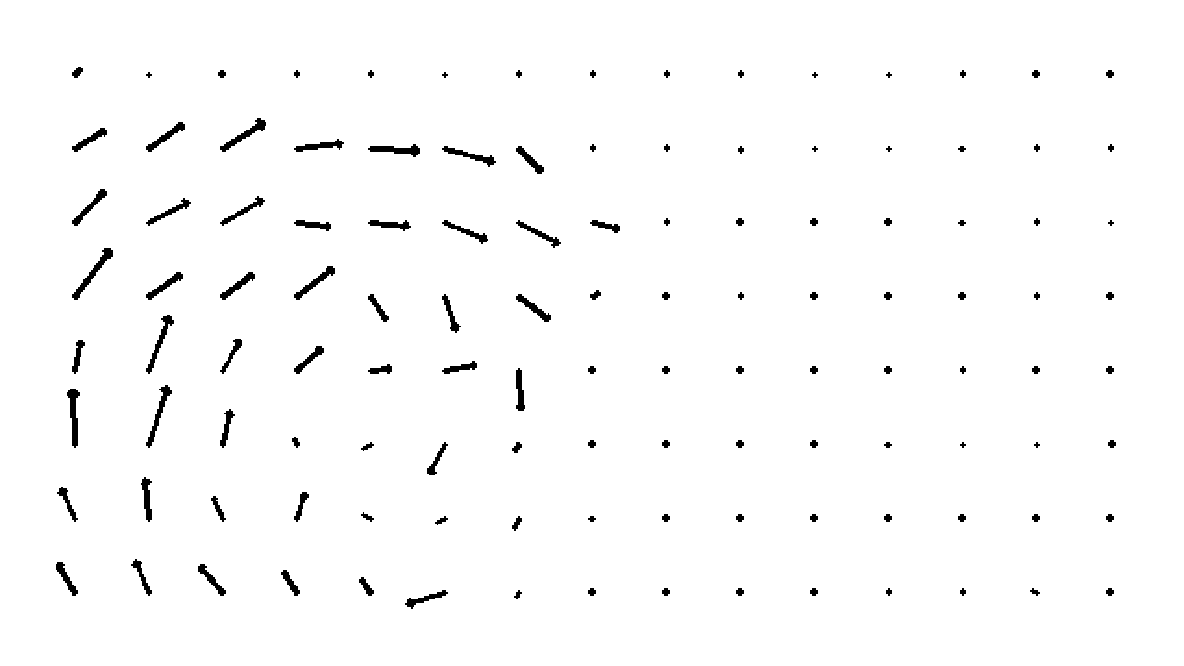
\includegraphics[width=7.5cm]{images/vectorField.png}
\end{figure}

\end{frame}

% --------------------
\begin{frame}[fragile]
\frametitle{Megvalósított funkciók}

\begin{columns}
	\begin{column}{4.5cm}
		\begin{block}{Gesztusok}
		\begin{itemize}
			\item Sweep
			\item Blink
			\item Drag and Drop
			\item Rotation
			\item (Többpontos kezelés)
			\item Symbol
		\end{itemize}
		\end{block}
	\end{column}
	
	\begin{column}{4.5cm}
		\begin{block}{Widgetek}
		\begin{itemize}
			\item Button
			\item Grabbable
			\item Shiftable
			\item Expandable
			\item Rollable
			\item Tuner
		\end{itemize}
		\end{block}
	\end{column}
\end{columns}

\begin{figure}[htb]
	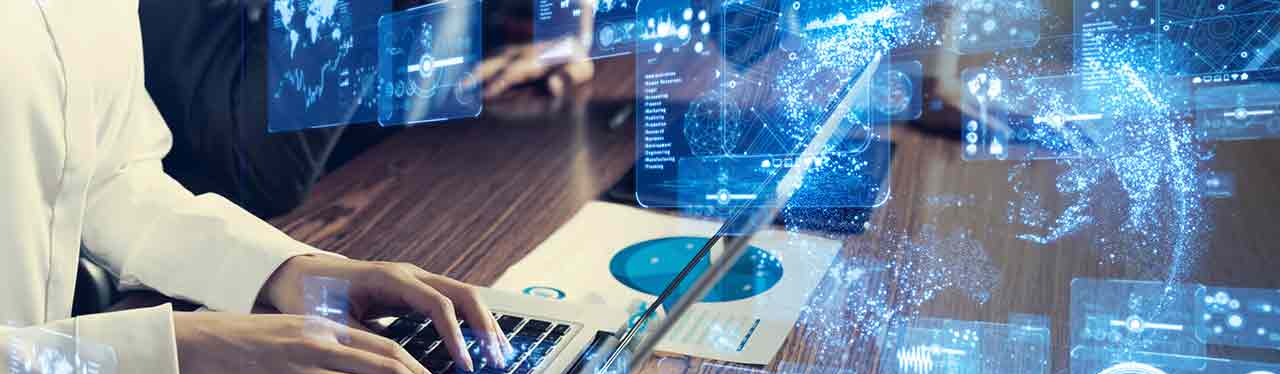
\includegraphics[width=\textwidth]{images/laptop.png}
\end{figure}

\end{frame}

% --------------------
\begin{frame}[fragile]
\frametitle{Felhasználási területek}

Elsősorban online felületeken történő alkalmazásra

\begin{itemize}
	\item Konferenciahívások
	\item Online előadások
	\item Élő közvetítések
\end{itemize}

\begin{figure}[htb]
	
\includegraphics[width=\textwidth]{images/virtual.png}
\end{figure}

\end{frame}

% --------------------
\begin{frame}[fragile]
\frametitle{Demo}

\begin{center}
	\Large
	\textbf{A program bemutatása Demoval}
\end{center}

\begin{figure}[htb]
	
\includegraphics[width=7cm]{images/demo.png}
\end{figure}

\end{frame}

% --------------------
\begin{frame}[fragile]
\frametitle{Irodalomjegyzék}

\bibliographystyle{plain}
\bibliography{Nagy_Daniel_prezentacio.bib}

\end{frame}

% --------------------
\begin{frame}[fragile]
\frametitle{\ }

\begin{center}
	\Large
	\textbf{Köszönöm szépen a figyelmet!}
\end{center}

\end{frame}

% --------------------


\end{document}
